\subsection{Identification Correct}
\label{sec:eval_req_id_correct} 

\subsubsection{Configuration}

\begin{figure}[H]
    \includegraphics[width=14cm,frame]{figures/eval_req_id_correct.png}
  \caption{Evaluation Identification Correct requirement}
\end{figure}

The 'Identification Correct' requirement is used to calculate the probability of a target report having a correct (secondary) identification. Correct in this context means there is identification data available, 
and it is the same as in the reference. \\

\begin{itemize}  
\item Probability [1]: Probability of correct identification
\item Probability Check Type: $\geq$
\item Require correctness of All: If checked, all available secondary attributes must match the reference. If not checked, a single matching secondary attribute is enough.
\item Use Mode 3/A Code: If the Mode 3/A code should be checked
\item Use Mode S Target Address: If the Mode S target address should be checked
\item Use Mode S Target Identification: If the Mode S target identification should be checked
\end{itemize}
\ \\

\subsubsection{Result Values}

\paragraph{Sector}

\begin{center}
 \begin{table}[H]
  \begin{tabularx}{\textwidth}{ | l | X |  l | }
    \hline
    \textbf{Name} & \textbf{Description} & \textbf{Example} \\ \hline
    Sector Layer & Name of the sector layer & fir\_cut\_sim \\ \hline
    Requirement Group & Name of the requirement group & Mandatory \\ \hline
    Requirement & Name of the requirement & Identification Correct \\ \hline
    Num Results & Total number of results & 728 \\ \hline
    Num Usable Results & Number of usable results & 107 \\ \hline
    Num Unusable Results & Number of unusable results & 621 \\ \hline
    \#Updates & Total number target reports & 101685 \\ \hline
    \#NoRef [1] & Number of updates w/o reference position or identification & 7359 \\ \hline
    \#NoRefPos [1] & Number of updates w/o reference position  & 7359 \\ \hline
    \#NoRef [1] & Number of updates w/o reference identification & 0 \\ \hline
    \#PosInside [1] & Number of updates inside sector & 53997 \\ \hline
    \#PosOutside [1] & Number of updates outside sector & 40329 \\ \hline
    \#CID [1] & Number of updates with correct identification & 53997 \\ \hline
    \#NCID [1] & Number of updates with no correct identification & 0 \\ \hline
    POK [\%] & Probability of correct identification & 100.00 \\ \hline
    Condition &  & >= 90.00 \\ \hline
    Condition Fulfilled &  & Passed \\ \hline
\end{tabularx}
\end{table}
\end{center}

Also, a table is given for all single targets, sorted by PEx.

\paragraph{Single Target}

\begin{center}
 \begin{table}[H]
  \begin{tabularx}{\textwidth}{ | l | X |  l | }
    \hline
    \textbf{Name} & \textbf{Description} & \textbf{Example} \\ \hline
    Use & To be used in results & true \\ \hline
    \#Up [1] & Number of updates & 892 \\ \hline
    \#NoRef [1] & Number of updates w/o reference position or identification & 84 \\ \hline
    \#NoRefPos [1] & Number of updates w/o reference position  & 84 \\ \hline
    \#NoRef [1] & Number of updates w/o reference identification & 0 \\ \hline
    \#PosInside [1] & Number of updates inside sector & 563 \\ \hline
    \#PosOutside [1] & Number of updates outside sector & 245 \\ \hline
    \#CID [1] & Number of updates with correct identification & 563 \\ \hline
    \#NCID [1] & Number of updates with no correct identification & 0 \\ \hline
    POK [\%] & Probability of correct identification & 100 \\ \hline
    Condition &  & >= 90.00 \\ \hline
    Condition Fulfilled &  & Passed \\ \hline
\end{tabularx}
\end{table}
\end{center}

\subsection{Identification Correct Periods}
\label{sec:eval_req_id_correct_periods} 

\subsubsection{Configuration}

\begin{figure}[H]
    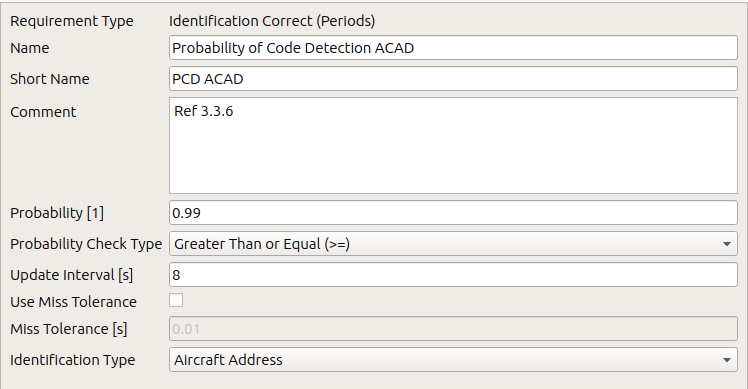
\includegraphics[width=14cm,frame]{figures/eval_req_id_correct_periods.png}
  \caption{Evaluation Identification Correct Periods requirement}
\end{figure}

This requirement calculates the probability of correct aircraft identification detection. \\

For each target existing in the reference data (within the current sector) a test target's identification should
be detected correctly within each test update interval. Correctly here means equality.
Update intervals without correct identification are counted as misses, which are used to calculate the probability of correct aircraft
identification detection, which has to fulfill a given threshold.

\begin{itemize}
    \item Probability [1]: Probability of correct aircraft identification detection
    \item Probability Check Type: $\geq$
    \item Update Interval [s]: Update interval of the test data
    \item Use Miss Tolerance: Checkbox if miss tolerance should be used
    \item Miss Tolerance [s]: Acceptable time delta for miss detection
    \item Identification Type: Type of identification to check (\textit{Aircraft Address}, \textit{Aircraft Identification} or \textit{Mode A})
\end{itemize}

\subsubsection{Result Values}

\paragraph{Sector}

\begin{center}
 \begin{table}[H]
  \begin{tabularx}{\textwidth}{ | l | X |  l | }
    \hline
    \textbf{Name} & \textbf{Description} & \textbf{Example} \\ \hline
    Sector Layer & Name of the sector layer & fir\_body\_cut \\ \hline
    Requirement Group & Name of the requirement group & En-Route \\ \hline
    Requirement & Name of the requirement & Probability of Code Detection ACAD \\ \hline
    Num Results & Total number of results & 317 \\ \hline
    Num Usable Results & Number of usable results & 81 \\ \hline
    Num Unusable Results & Number of unusable results & 236 \\ \hline
    \#Updates/\#EUIs [1] & Total number update intervals & 4265 \\ \hline
    \#MUIs [1] & Number of missed update intervals & 134 \\ \hline
    PCAAD [\%] & Probability of Correct Aircraft Address Detection & 96.86 \\ \hline
    Condition &  & >= 99.00 \\ \hline
    Condition Fulfilled &  & Failed \\ \hline
    \#Single Targets &  & 81 \\ \hline
    \#Failed Single Targets &  & 2 \\ \hline
\end{tabularx}
\end{table}
\end{center}

\paragraph{Single Target}

\begin{center}
 \begin{table}[H]
  \begin{tabularx}{\textwidth}{ | l | X |  l | }
    \hline
    \textbf{Name} & \textbf{Description} & \textbf{Example} \\ \hline
    Use & To be used in results & true \\ \hline
    \#EUIs [1] & Expected Update Intervals & 35 \\ \hline
    \#MUIs [1] & Missed Update Intervals & 0 \\ \hline
    PCAAD [\%] & Probability of Correct Aircraft Address Detection & 100 \\ \hline
    Reference Period 1 & Time inside sector & [2023-06-30 16:03:14.056,2023-06-30 16:07:57.236] \\ \hline
    Condition &  & >= 99.00 \\ \hline
    Condition Fulfilled &  & Passed \\ \hline
\end{tabularx}
\end{table}
\end{center}

\subsection{Identification False}
\label{sec:eval_req_id_false} 

\subsubsection{Configuration}

\begin{figure}[H]
    \includegraphics[width=14cm,frame]{figures/eval_req_id_false.png}
  \caption{Evaluation Identification False requirement}
\end{figure}

The 'Identification False' requirement is used to calculate the probability of a target report having a false (secondary) identification. False in this context means there is identification data available, and it is not the same as in the reference. \\

\begin{itemize}  
\item Probability [1]: Probability of false identification
\item Probability Check Type: $\leq$
\item Require All False: If checked, all available secondary attributes be different than in the reference to count. If not checked, a single wrong secondary attribute is enough.
\item Use Mode 3/A Code: If the Mode 3/A code should be checked
\item Use Mode S Target Address: If the Mode S target address should be checked
\item Use Mode S Target Identification: If the Mode S target identification should be checked
\end{itemize}
\ \\

\subsubsection{Result Values}

\paragraph{Sector}

\begin{center}
 \begin{table}[H]
  \begin{tabularx}{\textwidth}{ | l | X |  l | }
    \hline
    \textbf{Name} & \textbf{Description} & \textbf{Example} \\ \hline
    Sector Layer & Name of the sector layer & fir\_cut\_sim \\ \hline
    Requirement Group & Name of the requirement group & Mandatory \\ \hline
    Requirement & Name of the requirement & Identification False \\ \hline
    Num Results & Total number of results & 728 \\ \hline
    Num Usable Results & Number of usable results & 107 \\ \hline
    Num Unusable Results & Number of unusable results & 621 \\ \hline
    Use & To be used in results & true \\ \hline
    \#Up [1] & Number of updates & 101685 \\ \hline
    \#NoRef [1] & Number of updates w/o reference position or identification & 7359 \\ \hline
    \#NoRefPos [1] & Number of updates w/o reference position  & 7359 \\ \hline
    \#NoRef [1] & Number of updates w/o reference identification & 0 \\ \hline
    \#PosInside [1] & Number of updates inside sector & 53997 \\ \hline
    \#PosOutside [1] & Number of updates outside sector & 40329 \\ \hline
    \#Unknown [1] & Number of updates unknown identification & 0 \\ \hline
    \#Correct [1] & Number of updates with correct identification & 53997 \\ \hline
    \#False [1] & Number of updates with false identification & 0 \\ \hline
    PF [\%] & Probability of identity false & 0 \\ \hline
    Condition &  & <= 1.00 \\ \hline
    Condition Fulfilled &  & Passed \\ \hline
\end{tabularx}
\end{table}
\end{center}

Also, a table is given for all single targets, sorted by PF.

\paragraph{Single Target}

\begin{center}
 \begin{table}[H]
  \begin{tabularx}{\textwidth}{ | l | X |  l | }
    \hline
    \textbf{Name} & \textbf{Description} & \textbf{Example} \\ \hline
    Use & To be used in results & true \\ \hline
    \#Up [1] & Number of updates & 566 \\ \hline
    \#NoRef [1] & Number of updates w/o reference position or identification & 51 \\ \hline
    \#NoRefPos [1] & Number of updates w/o reference position  & 51 \\ \hline
    \#NoRef [1] & Number of updates w/o reference identification & 0 \\ \hline
    \#PosInside [1] & Number of updates inside sector & 292 \\ \hline
    \#PosOutside [1] & Number of updates outside sector & 223 \\ \hline
    \#Unknown [1] & Number of updates unknown identification & 0 \\ \hline
    \#Correct [1] & Number of updates with correct identification & 292 \\ \hline
    \#False [1] & Number of updates with false identification & 0 \\ \hline
    PF [\%] & Probability of Mode 3/A false & 0 \\ \hline
    Condition &  & <= 1.00 \\ \hline
    Condition Fulfilled &  & Passed \\ \hline
\end{tabularx}
\end{table}
\end{center}
